\documentclass[12pt,a4paper]{article}
\usepackage{graphicx,textcomp}
\usepackage{natbib}
\usepackage{setspace}
\usepackage{fullpage}
\usepackage{color}
\usepackage[reqno]{amsmath}
\usepackage{amsthm}
\usepackage{fancyvrb}
\usepackage{amssymb,enumerate}
\usepackage[all]{xy}
\usepackage{endnotes}
\usepackage{lscape}
\newtheorem{com}{Comment}
\usepackage{float}
\usepackage{hyperref}
\newtheorem{lem} {Lemma}
\newtheorem{prop}{Proposition}
\newtheorem{thm}{Theorem}
\newtheorem{defn}{Definition}
\newtheorem{cor}{Corollary}
\newtheorem{obs}{Observation}
\usepackage[compact]{titlesec}
\usepackage{dcolumn}
\usepackage{tikz}
\usetikzlibrary{arrows}
\usepackage{multirow}
\usepackage{xcolor}
\usepackage{adjustbox}
\newcolumntype{.}{D{.}{.}{-1}}
\newcolumntype{d}[1]{D{.}{.}{#1}}
\definecolor{light-gray}{gray}{0.65}
\usepackage{url}
\usepackage{listings}
\usepackage{color}

\definecolor{codegreen}{rgb}{0,0.6,0}
\definecolor{codegray}{rgb}{0.5,0.5,0.5}
\definecolor{codepurple}{rgb}{0.58,0,0.82}
\definecolor{backcolour}{rgb}{0.95,0.95,0.92}

\lstdefinestyle{mystyle}{
	backgroundcolor=\color{backcolour},   
	commentstyle=\color{codegreen},
	keywordstyle=\color{magenta},
	numberstyle=\tiny\color{codegray},
	stringstyle=\color{codepurple},
	basicstyle=\footnotesize,
	breakatwhitespace=false,         
	breaklines=true,                 
	captionpos=b,                    
	keepspaces=true,                 
	numbers=left,                    
	numbersep=5pt,                  
	showspaces=false,                
	showstringspaces=false,
	showtabs=false,                  
	tabsize=2
}
\lstset{style=mystyle}
\newcommand{\Sref}[1]{Section~\ref{#1}}
\newtheorem{hyp}{Hypothesis}

\title{Predicting House Prices}
\date{Conor, Linette, Lucas, Minh}
\author{Quantitative Methods 1 (Tutorial)}

\begin{document}

\maketitle

\section{Variable selection}

	\noindent To predict the Adjusted Sale Price of houses, we considered three major factors:
	
	\begin{itemize}
		\item the neighbourhood;
		\item the size of the house; and
		\item the quality of the construction. \\
	\end{itemize}
	
	\noindent Figure 1 below summarizes the variables we selected to represent each of those characteristics and their relationship.
	
	\begin{figure}[H]
		\centering
		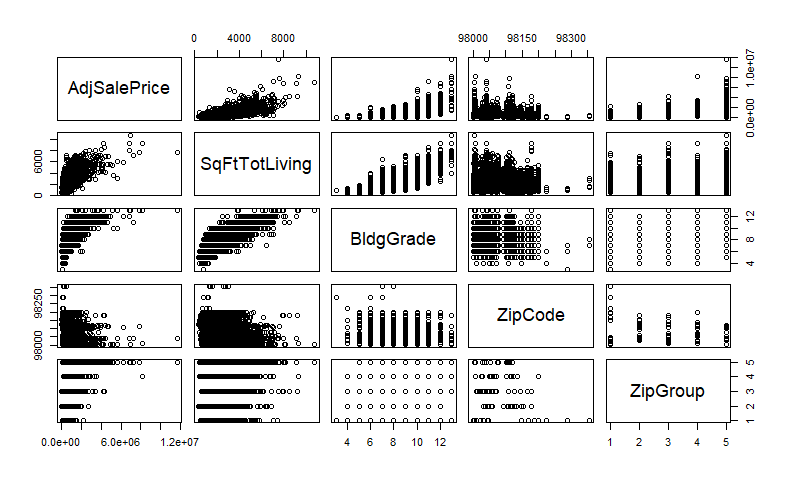
\includegraphics[width=1\linewidth]{AdjSalePrice_pairs}
		\caption{Associations of \texttt{AdjSalePrice} with \texttt{SqFtTotLiving}, \texttt{BldgGrade}, and \texttt{ZipCode}}
		\label{fig:adjsalepricepairs}
	\end{figure}
		
	\noindent \texttt{ZipCode} represents \textbf{neighborhood}. We grouped zip codes based on house prices in the variable \texttt{ZipGroup} to reflect the socioeconomic profile of each neighborhood. \\
	
	\noindent \texttt{SqFtTotLiving} represents the \textbf{size of the house}. We avoided adding to the model the variables \texttt{SqFtLot}, \texttt{SqFtFinBasement}, \texttt{NbrLivingUnits} \texttt{Bathrooms}, and \texttt{Bedrooms} because they are also related to the size of the construction. That decision allowed us to reach a more \textbf{parsimonious} model, preventing us from loosing degrees of freedom and from incurring in issues related to \textbf{collinearity}. The risk of collinearity among those variables is visible in Figure 2 below: \\
	
	\begin{figure}[H]
		\centering
		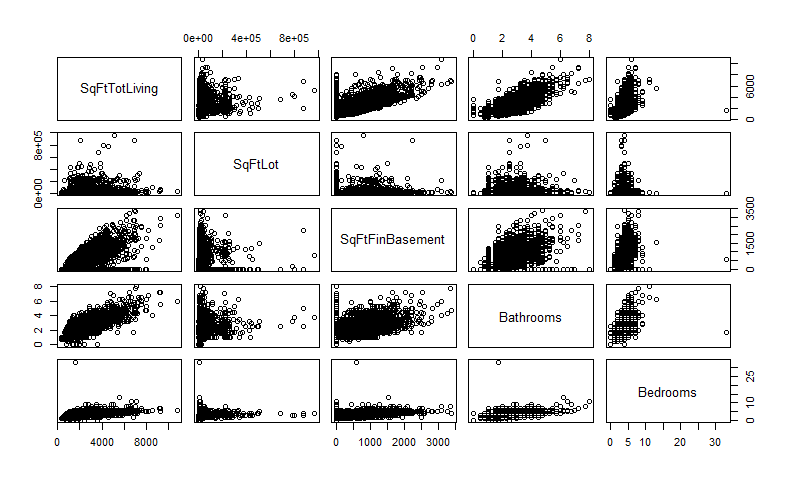
\includegraphics[width=1\linewidth]{SqFtTotLiving_pairs}
		\caption{Risk of collinearity among \texttt{SqFtLot}, \texttt{SqFtFinBasement}, \texttt{Bathrooms}, and \texttt{Bedrooms}}
		\label{fig:sqfttotlivingpairs}
	\end{figure}
		
	\noindent Lastly, \texttt{BldgGrade} represents the \textbf{quality of the construction}. For the same reasons stated above (parsimony, preventing the loss of degrees of freedom, and avoiding collinearity issues), we decided not to add \texttt{YrBuilt}, \texttt{YrRenovated}, and \texttt{NewConstruction}, which are also related to the quality of the construction. \\
	
\vspace{.5cm}

\section{Interaction effect}

	To complete the model, we added an interaction effect between \texttt{ZipGroup} and \texttt{SqFtTotLiving}. The interaction reflects the idea that each additional square foot in the building will affect house prices differently depending on the neighborhood. As a consequence, the slope of \texttt{SqFtTotLiving} on \texttt{AdjSalePrice} in expensive neighborhoods will be steeper than in popular ones.

\vspace{.5cm}

\section{Final model}

\end{document}
